\begin{frame}
	\frametitle{I linguaggi di codifica}
	\framesubtitle{introduzione}
	\addtocounter{nframe}{1}

	\begin{block}{Definizione di codifica digitale del testo}
		Per \textbf{codifica} digitale dei testi intendiamo la \textit{rappresentazione formale} di un \textbf{testo} ad un qualche livello descrittivo, su di un supporto digitale, in un formato utilizzabile da un elaboratore (\textit{Machine Readable Form}) mediante un opportuno \textbf{linguaggio informatico} (F. Ciotti).
	\end{block}

\end{frame}

\begin{frame}
	\frametitle{Markup language e XML}
	\framesubtitle{soluzione corrente per la codifica dei testi}
	\addtocounter{nframe}{1}

	\begin{block}{XML per la descrizione e la codifica}
		Ad oggi la soluzione considerata ottimale per una corretta rappresentazione del testo è l'adozione dei markup language descrittivi basati su XML.
	\end{block}

\end{frame}

\begin{frame}
	\frametitle{I linguaggi di codifica}
	\framesubtitle{Linguaggi di marcatura}
	\addtocounter{nframe}{1}

	\begin{block}{Il markup}
		Il termine \textbf{markup} è stato utilizzato in passato per denotare i \textbf{segni grafici} che accompagnavano un testo apposti sul documento per \textbf{indicare correzioni o modalità grafiche di stampa}.
	\end{block}

\end{frame}

\begin{frame}
	\frametitle{I linguaggi di codifica}
	\framesubtitle{Linguaggi di marcatura}
	\addtocounter{nframe}{1}

	\begin{center}
		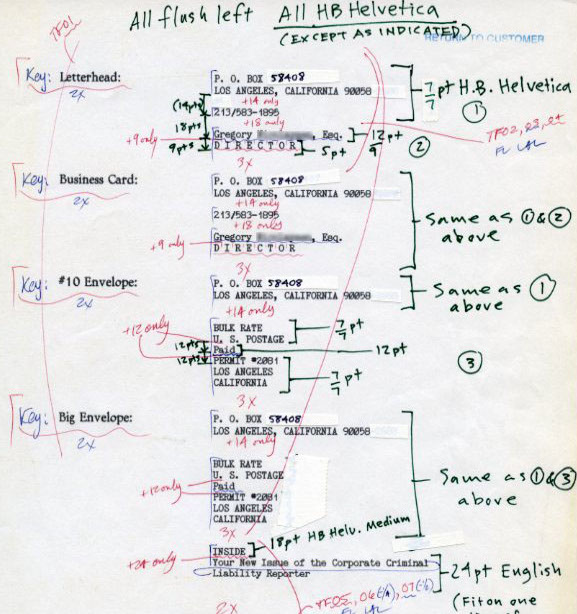
\includegraphics[width=.6\textwidth]{imgs/xml-markup001.jpg}
	\end{center}

\end{frame}

\begin{frame}
	\frametitle{I linguaggi di codifica}
	\framesubtitle{Linguaggi di marcatura}
	\addtocounter{nframe}{1}

	\begin{center}
		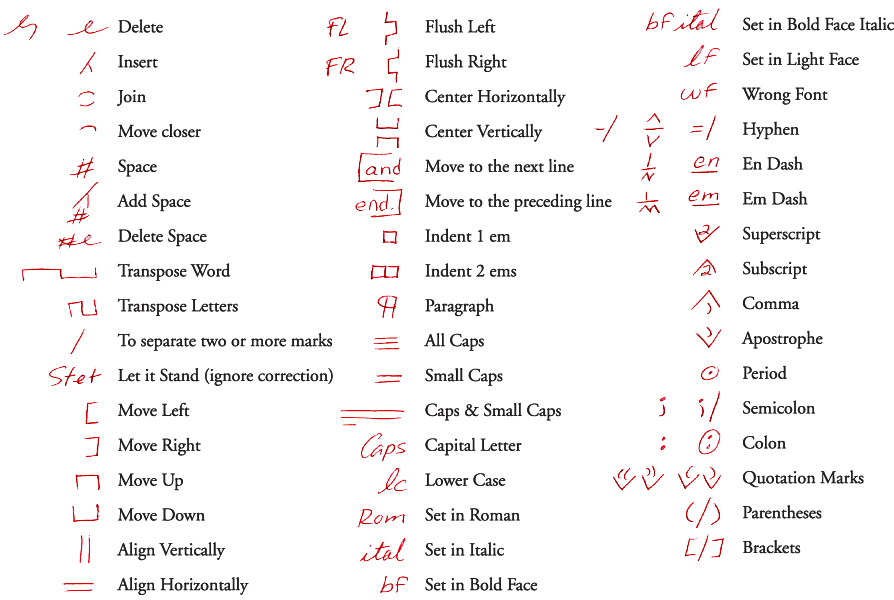
\includegraphics[width=.9\textwidth]{imgs/xml-MarkupConvention.png}
	\end{center}

\end{frame}

\begin{frame}
	\frametitle{I linguaggi di codifica}
	\framesubtitle{Linguaggi di marcatura}
	\addtocounter{nframe}{1}

	\begin{block}{Il markup}
		La codifica con linguaggi di marcatura (markup) è in sostanza \textbf{un insieme di convenzioni}, rese attraverso specifiche \textbf{sequenze di caratteri, etichette, codici}, (detti \textit{tags}) \textbf{intercalati nel testo} per permettere agli elaboratori elettronici di distinguere le varie parti di un documento.
	\end{block}

	\begin{block}{Il markup formale}
		Un linguaggio di markup è un \textbf{sistema formale} per \textit{scambiare} e \textit{pubblicare} informazioni in \textbf{formato testo in modo strutturato}.
	\end{block}


\end{frame}

%slide relative ad introdurre gli elementi di XML

% prendere da libro XML in amazon e XML visual quick view
% inserire qualche nota sul namespace anche preso dal libro xsd da pag 26 
% riprendere qualche slide dall slide Del Turco; e dalle slide Fiormonte-Ciotti-Silvi-XML-corso-2014.pdf
% http://filologiadigitale-verona.it/wp-content/uploads/2014/10/Fiormonte-Ciotti-Silvi-XML-corso-2014.pdf
% Slide Chiara di Pietro

% IDE/Editor comes with a nice XML/XSD editor. It has a number of features that makes schema writing lot easier. Intellisense, auto-completion, real-time syntax checks, etc., are a few of those features.

\begin{frame}
	\frametitle{Fondamenti XML}
	\framesubtitle{eXtensible Markup Language}
	\addtocounter{nframe}{1}

	\begin{block}{XML origini}
		XML affonda le proprie origini nel linguaggio \textbf{Standard Generalized Markup Language} (\textit{SGML}).
		\\ SGML è stato introdotto negli anni ottanta con il fine di \textbf{descrivere la struttura e il contenuto di qualsiasi informazione} ``machine readable''.
	\end{block}

	\begin{block} {XML è una semplificazione di SGML}
		XML può essere pensato come una \textbf{versione semplificata di SGML}. Infatti, come SGML, \textit{XML è un meta-linguaggio}, usato per \textit{create linguaggi di marcatura} (detti \textbf{vocabolari}).
	\end{block}
\end{frame}

\begin{frame}
	\frametitle{Fondamenti XML}
	\framesubtitle{eXtensible Markup Language}
	\addtocounter{nframe}{1}

	\begin{block}{XML come meta-linguaggio}
		XML, \textit{eXtensible Markup Language}, \textbf{è un insieme di regole} per definire linguaggi di marcatura personalizzati e personalizzabili (\textit{custom-built vocabolaries}).
	\end{block}

	\begin{block} {Applicazioni XML}
		Allo stesso modo di SGML, XML è nato per \textbf{strutturare}, \textbf{conservare} e \textbf{trasportare} informazioni.
		\\ I linguaggi di marcatura derivati da XML per strutturare e descrivere specifiche informazioni vengono chiamati \textit{XML applications} oltre che \textit{vocabolario XML}.
	\end{block}
\end{frame}

\begin{frame}
	\frametitle{Fondamenti XML}
	\framesubtitle{eXtensible Markup Language}
	\addtocounter{nframe}{1}

	\begin{block}{XML: eXtensible}
		XML è \textbf{estensibile}: è pensato per essere \textit{modificato} ed \textit{esteso} al fine di soddisfare le varie necessità di rappresentazione dell'informazione.
		\textbf{XML non contempla un vocabolario predefinito!}
	\end{block}

	\begin{block} {XML: standard W3C}
		XML è sviluppato e \textbf{manutenuto dal W3C} (World Wide Web Consortium), il quale sviluppa \textit{protocolli} e \textit{standard} riconosciuti dalla comunità scientifica e tecnica al fine di \textbf{condividere informazioni sul Web}.
	\end{block}
\end{frame}

\begin{frame}
	\frametitle{Fondamenti XML}
	\framesubtitle{eXtensible Markup Language}
	\addtocounter{nframe}{1}

	\begin{block}{XML: riassumendo}
		XML, eXtensible Markup Language, deriva da SGML ed 
		è una \textbf{specificazione}, un \textbf{formalismo}, per \textit{strutturare}, \textit{conservare} e \textit{scambiare} informazioni in formato machine readable (\textit{digitale}).
	\end{block}

	\begin{block}{XML: riassumendo}
		XML è anche una specificazione per \textbf{descrivere la struttura dell'informazione} seguendo un \textbf{modello dei dati gerarchico}.
		\\ XML è simile ad HTML, ma a differenza di questo non ha etichette predefinite.
	\end{block}

\end{frame}


\begin{frame}
	\frametitle{Fondamenti XML}
	\framesubtitle{eXtensible Markup Language}
	\addtocounter{nframe}{1}

	\begin{center}
		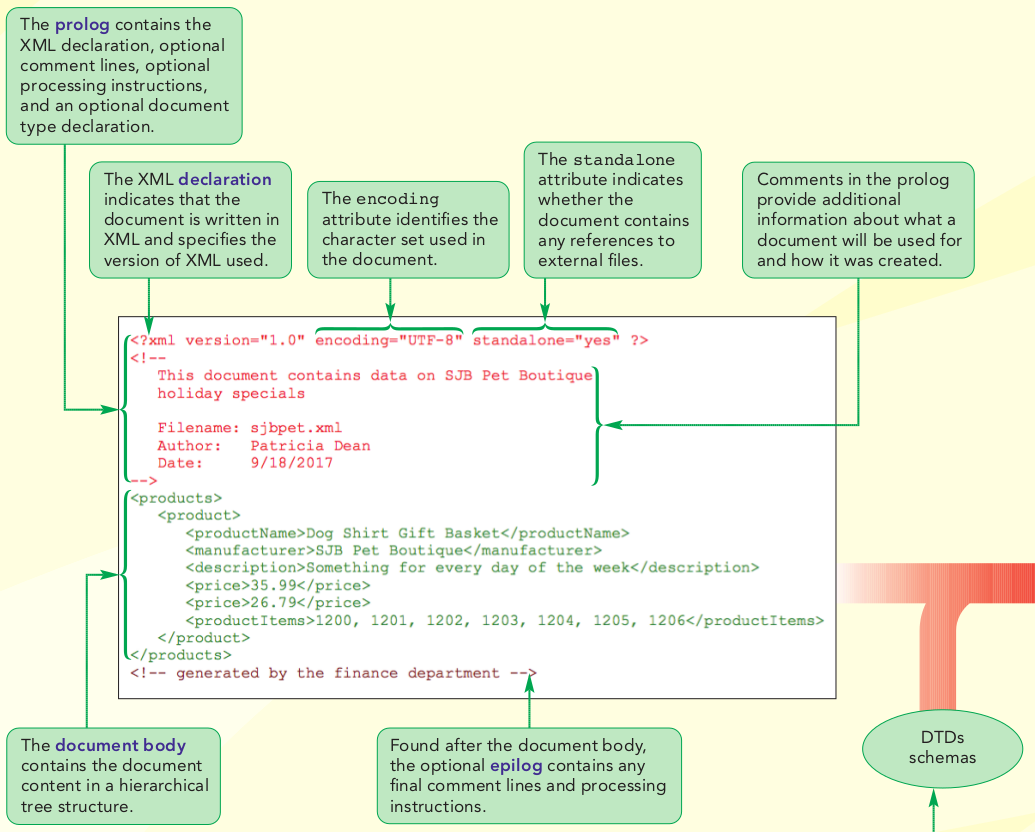
\includegraphics[width=.8\textwidth]{imgs/xml-intro-doc-xml.png}
	\end{center}

	\begin{tiny}\textit{immagine dal libro New Perspectives on XML, 3rd Edition}\end{tiny}

\end{frame}


%The syntax rules of XML are easy to learn and easy to use
\begin{frame}
	\frametitle{Fondamenti XML}
	\framesubtitle{eXtensible Markup Language: regole sintattiche}
	\addtocounter{nframe}{1}

	\begin{itemize}

		\item Ciascun elemento XML deve avere un tag di chiusura.
			%Every XML element must have a closing tag.
		      %Every element must have a closing tag. A self-closing tag is permitted.

		\item I tag XML sono \textit{case sensitive}.
			%XML tags are case sensitive.
		      % Opening and closing tags (or start and end tags) must be ­written with the same case.

		\item Gli elementi XML devono essere annidati in modo rigoroso.
			%XML elements must be ­properly nested.
		      %All elements can have child (sub) elements. Child elements must be in pairs and be correctly nested within their respective parent element.

		\item Tutti i documenti XML deveno avere un elemento radice (root) che contiene tutti gli altri elementi opportunamente annidati.
			%Every XML document must have a root element.
		      %Every XML document must contain a single tag pair that defines the root element. All other elements must be nested within the root element.

		\item Gli elementi XML possono avere attributi con stile nome-valore.
		
	\end{itemize}

\end{frame}


%The syntax rules of XML are easy to learn and easy to use 2
\begin{frame}
	\frametitle{Fondamenti XML}
	\framesubtitle{eXtensible Markup Language: regole sintattiche cont.}
	\addtocounter{nframe}{1}

	\begin{itemize}
		\item Un attributo all'interno dell'elemento può apparire una sola volta
		
		\item Il valore degli attributi è una stringa e deve essere inserita tra apici
			%XML elements can have attributes in name-value pairs.
		      %Each attribute name within the same element can occur only once.% Each attribute value must be quoted.

		\item Esistono alcuni caratteri speciali che non possono essere usati. 
			%Some characters have a ­special meaning in XML.
		      %The use of certain characters is restricted. If these characters are needed, entity references or character references may be used. References always begin with the character “&” (which is ­specially reserved) and end with the character “;”.

		      %XML allows for comments. 
		\item I commenti non possono essere inseriti prima della dichiarazione XML e non possono essere annidati.
			%Comments cannot occur prior to the XML Declaration. Comments cannot be nested.

	\end{itemize}

\end{frame}

\begin{frame}
	\frametitle{Fondamenti XML}
	\framesubtitle{eXtensible Markup Language}
	\addtocounter{nframe}{1}

	\begin{block}{Manutenibilità}
		Data la semplicità delle regole e della sintassi XML incentrata sulla memorizzazione e scambio dei dati, la struttura generale di un documento XML è semplice sia dal punto di vista della progettazione sia dal punto di vista della manutenibilità.
	\end{block}

\end{frame}

\begin{frame}
	\frametitle{Fondamenti XML}
	\framesubtitle{eXtensible Markup Language}
	\addtocounter{nframe}{1}

	\begin{block}{XML vista ad albero}
		XML ha un modello dei dati gerarchico e può quindi essere visto come un albero ordinato.
		\\Per questo motivo le informazioni sono rappresentate in modo ottimale se sono gerarchiche e sequenziali.
	\end{block}

\end{frame}


\begin{frame}
	\frametitle{Fondamenti XML}
	\framesubtitle{eXtensible Markup Language: vista ad albero}
	\addtocounter{nframe}{1}

	\begin{center}
		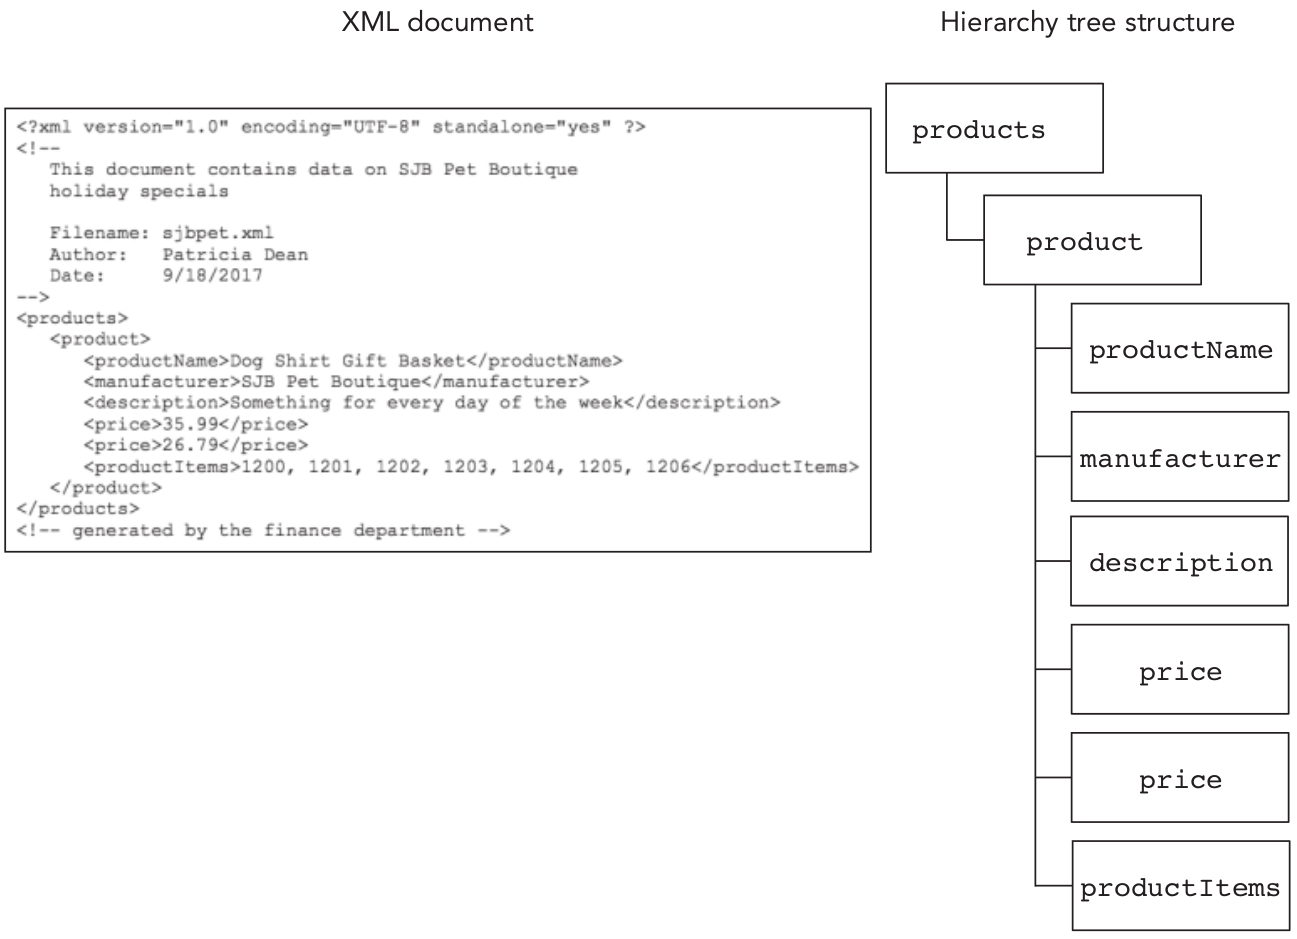
\includegraphics[width=.9\textwidth]{imgs/XML-TreeStructure.png}
	\end{center}

\begin{tiny}\textit{immagine dal libro New Perspectives on XML, 3rd Edition}\end{tiny}

\end{frame}

\begin{frame}
	\frametitle{Fondamenti XML}
	\framesubtitle{eXtensible Markup Language}
	\addtocounter{nframe}{1}

	\begin{block}{TEI-XML vocabulary}
		Al fine di soddisfare i \textbf{requisiti degli studiosi del testo} il \textit{vocabolario TEI-XML} è stato sviluppato nel corso degli ultimi decenni con lo scopo e l'obiettivo di \textit{permettere la codifica di qualsiasi informazione testuale}.
	\end{block}
	
	\textit{Un vocabolario XML è un insieme di tag XML sviluppato per una particolare esigenza di codifica}

\end{frame}


\begin{frame}
	\frametitle{Fondamenti XML}
	\framesubtitle{eXtensible Markup Language: Esempio TEI}
	\addtocounter{nframe}{1}

	\begin{center}
		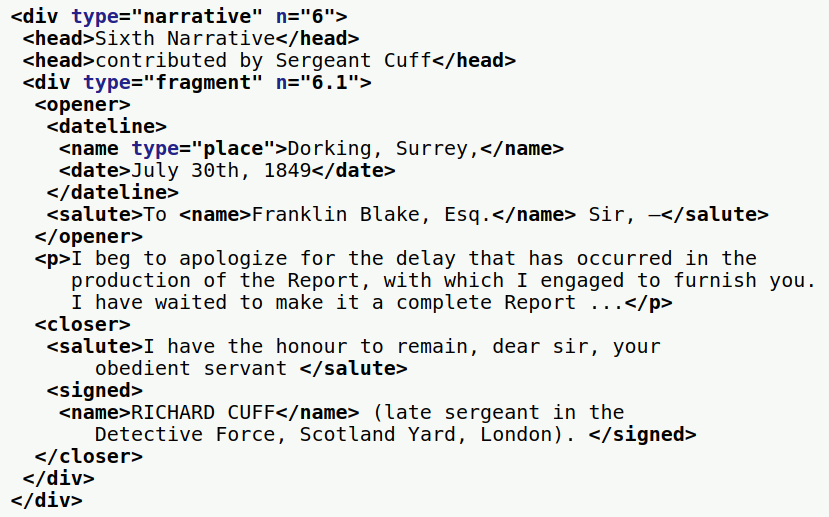
\includegraphics[width=.9\textwidth]{imgs/xml-TEI-Example.png}
	\end{center}

	\begin{tiny}
        \textit{immagine dal sito TEI Guide Lines}
    \end{tiny}

\end{frame}


\begin{frame}
	\frametitle{Fondamenti XML}
	\framesubtitle{eXtensible Markup Language}
	\addtocounter{nframe}{1}

	\begin{block}{Documento ben formato (well-formed)}
		Un documento XML deve essere \textbf{ben formato} (\textit{well-formed},cioè non deve contenere \textbf{errori sintattici} e deve soddisfare le \textbf{regole generali della specifica}.
	\end{block}
	\textit{Un documento non ben formato non può essere letto dalle applicazioni che elaborano codice XML}.

\end{frame}


\begin{frame}
	\frametitle{Fondamenti XML}
	\framesubtitle{eXtensible Markup Language}
	\addtocounter{nframe}{1}

	\begin{block}{Parti principali di un documento XML}
		Un documento XML consiste di tre parti:
		\begin{itemize}
			\item il prologo
			\item il corpo (body)
			\item l'epilogo
		\end{itemize}
	\end{block}

\end{frame}


\begin{frame}
	\frametitle{Fondamenti XML}
	\framesubtitle{eXtensible Markup Language: Esempio TEI}
	\addtocounter{nframe}{1}

	\begin{center}
		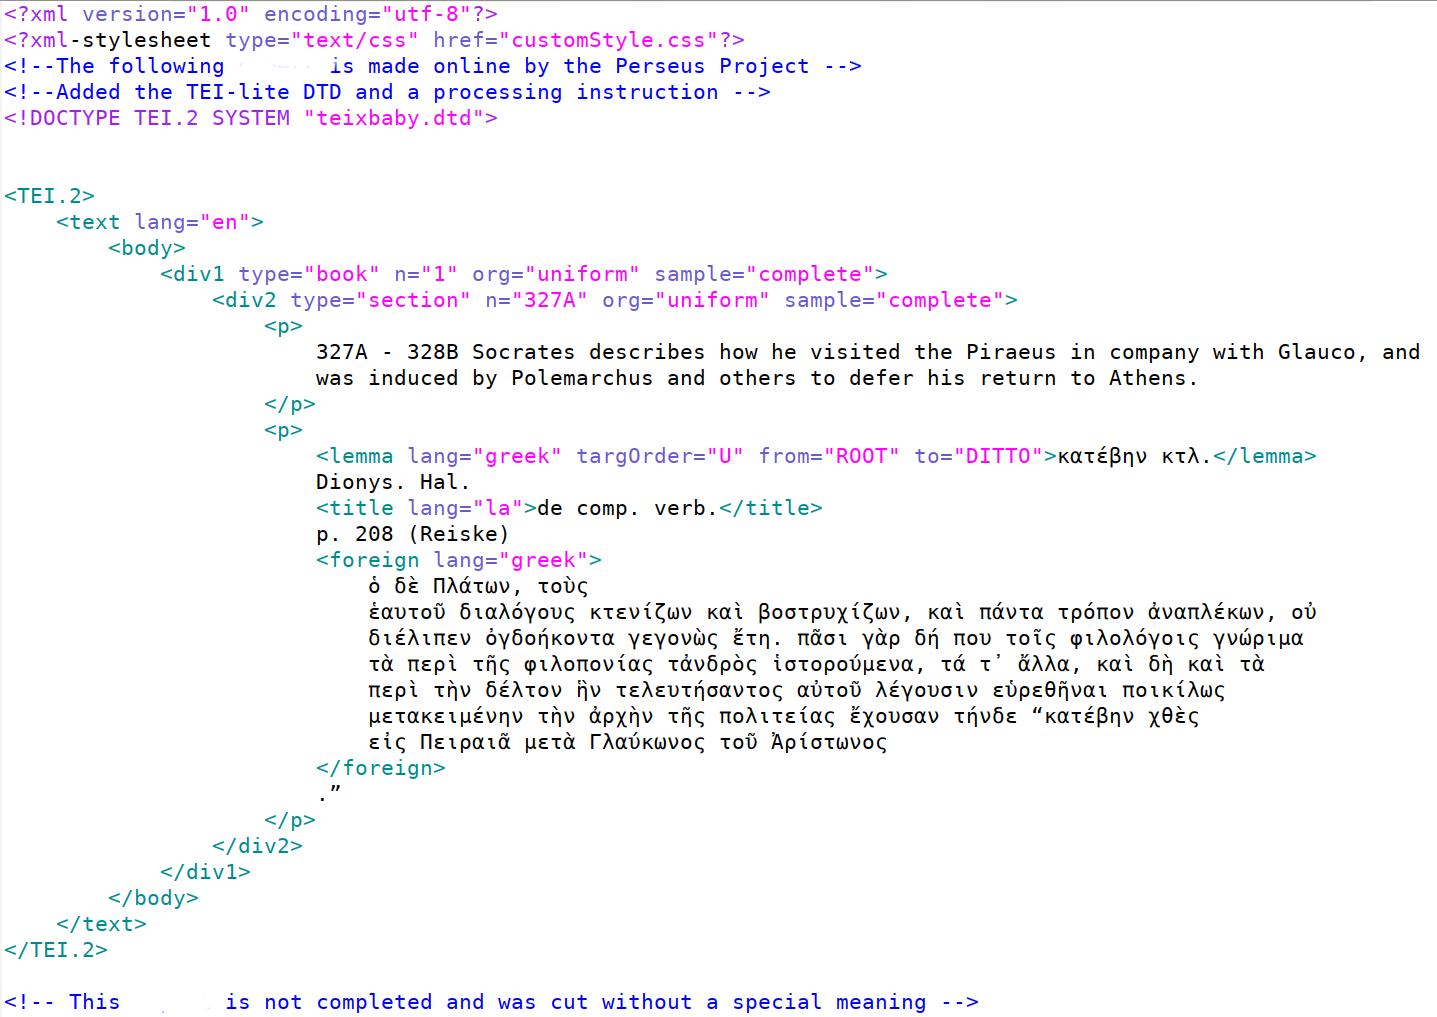
\includegraphics[width=0.95\textwidth]{imgs/xml-TEI-PerseusExample.png}
	\end{center}

\end{frame}


\begin{frame}
	\frametitle{Fondamenti XML}
	\framesubtitle{eXtensible Markup Language}
	\addtocounter{nframe}{1}

	\begin{block}{Documento XML: prologo}
		\begin{itemize}
			\item XML declaration (obbligatorio)
			\item Processing instructions (opzionale)
			\item Commenti (opzionale)
			\item Document type declaration (opzionale)
		\end{itemize}
        
        % XML declaration: indicates that the document is written in the XML language
        % Processing instructions (optional): provide additional instructions to be run by programs that read the XML document
        % Comment lines (optional): provide additional information about the document contents
        % Document type declaration (DTD) (optional): provides information about the rules used in the XML document’s vocabulary
	\end{block}

\end{frame}

\begin{frame}
	\frametitle{Fondamenti XML}
	\framesubtitle{eXtensible Markup Language}
	\addtocounter{nframe}{1}

	\begin{block}{Documento XML: corpo}
		Il corpo del documento XML segue immediatamente il prologo. Questa parte del documento contiene il contenuto vero e proprio in una \textbf{struttura ad albero ordinata}.
	\end{block}

	\begin{block}{Documento XML: epilogo}
		Opzionalmente, al corpo del documento XML segue un epilogo il quale può contenere commenti finali e processing instructions.
	\end{block}
	

\end{frame}

\begin{frame}
	\frametitle{Fondamenti XML}
	\framesubtitle{eXtensible Markup Language: Prologo}
	\addtocounter{nframe}{1}

	\begin{block}{XML declaration}
    \begin{center}\texttt{<?xml version=”version number” encoding=”encoding type” standalone=”yes|no” ?>}\end{center}
	\end{block}

\end{frame}

% Creating an XML Declaration
% • To create an XML declaration, enter the code
% <?xml ?>
% in the first line of an XML document.
% • To specify a version of XML to use, enter the code
% version=”version number”
% after the opening <?xml tag, where version number is either 1.0 or 1.1.
% • To specify a character encoding, enter the code
% encoding=”encoding type”
% after the version attribute-value pair, where encoding type identifies the ­character
% set used in the document.
% • To indicate whether the document is a standalone document, enter the code
% standalone=”yes|no”
% after the encoding attribute-value pair, where the value yes or no ­indicates whether
% access to external files will be needed when processing the document.

\begin{frame}
	\frametitle{Fondamenti XML}
	\framesubtitle{eXtensible Markup Language: Prologo}
	\addtocounter{nframe}{1}

	\begin{block}{XML declaration: ERRORI}
	\begin{center}\texttt{<?XML VERSION=”1.0” ENCODING=”ISO-8859-1” STANDALONE=”YES” ?>}\end{center}
	\begin{center}\texttt{<?xml version=1.0 encoding=ISO-8859-1 standalone=yes ?>}\end{center}
	\begin{center}\texttt{<?xml version=”1.0” standalone=”yes” encoding=”ISO-8859-1” ?>}\end{center}
	\end{block}

\end{frame}

\begin{frame}
	\frametitle{Fondamenti XML}
	\framesubtitle{eXtensible Markup Language: Prologo}
	\addtocounter{nframe}{1}

	\begin{block}{XML comments}
		I commenti XML vengono ignorati dai programmi che elaborano il documento.
		\\I commenti quindi non influenzano i contenuti e la struttura del documento.
	\end{block}

	\begin{block}{XML comments: sintassi}
	\begin{center}\texttt{
		<!-- il parser XML qui non entra -->
	}\end{center}
	\end{block}

	\textit{Un commento può occupare anche più righe}
	
\end{frame}

\begin{frame}
	\frametitle{Fondamenti XML}
	\framesubtitle{eXtensible Markup Language}
	\addtocounter{nframe}{1}

	\begin{center}
		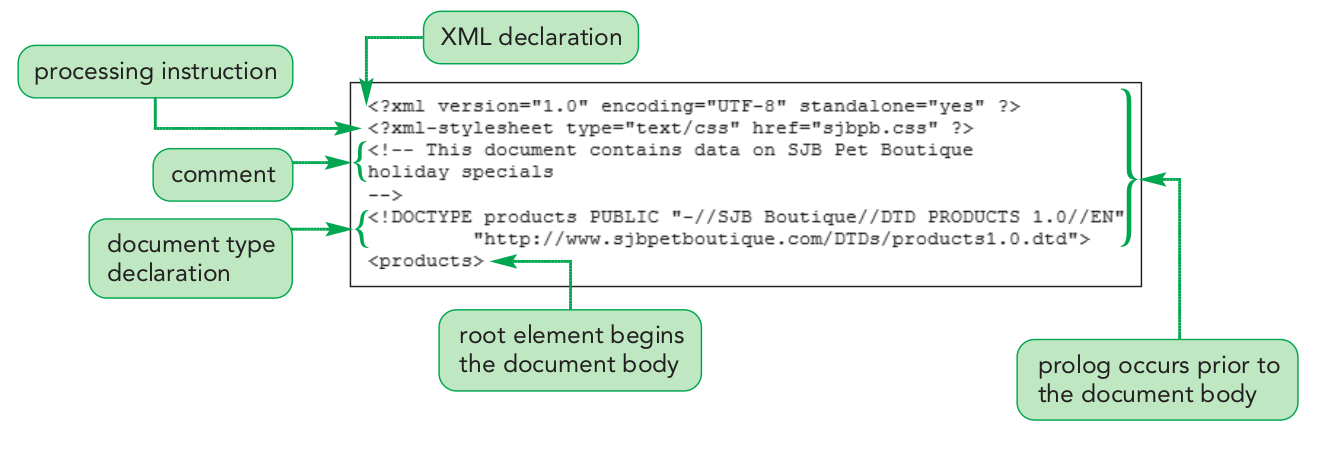
\includegraphics[width=0.95\textwidth]{imgs/XML-Prologo.png}
    \end{center}
\begin{tiny}\textit{immagine dal libro New Perspectives on XML, 3rd Edition}\end{tiny}

\end{frame}

\begin{frame}
	\frametitle{Fondamenti XML}
	\framesubtitle{eXtensible Markup Language}
	\addtocounter{nframe}{1}

	\begin{block}{Esercizio prologo}
		Creare un file \textit{.xml} ed inserire un prologo con la dichiarazione XML e un commento con le vostre informazioni.
	\end{block}

	\begin{block}{Esercizio prologo}
		\texttt{
		 <!--
		 	This document contains data on Codifica di Testi.
		 	\\Filename: project.xml
		 	\\Author: your name
		 	\\Date: today's date
		-->
		}
	\end{block}

	\begin{tiny}
		\textit{Salvare il file su github nel repository del progetto}
	\end{tiny}

\end{frame}

\begin{frame}
	\frametitle{Fondamenti XML}
	\framesubtitle{eXtensible Markup Language}
	\addtocounter{nframe}{1}

	\begin{block}{XML parser}
		Un programma che legge ed interpreta un documento XML è chiamato XML parser ( o processor).
	\end{block}
	\begin{block}{Cosa fa un XML parser}
		\begin{itemize}
			\item Verifica che il documento rispetti la sintassi XML
			\item Interpreta i dati con tipo PCDATA (\textit{Parsed})
			\item Risolve character or entity references
			\item Gestisce le processing instructions per interpretare i dati
		\end{itemize}
	\end{block}

\end{frame}

\begin{frame}
	\frametitle{Fondamenti XML}
	\framesubtitle{eXtensible Markup Language}
	\addtocounter{nframe}{1}

	\begin{block}{XMLlint}
		\begin{center}
			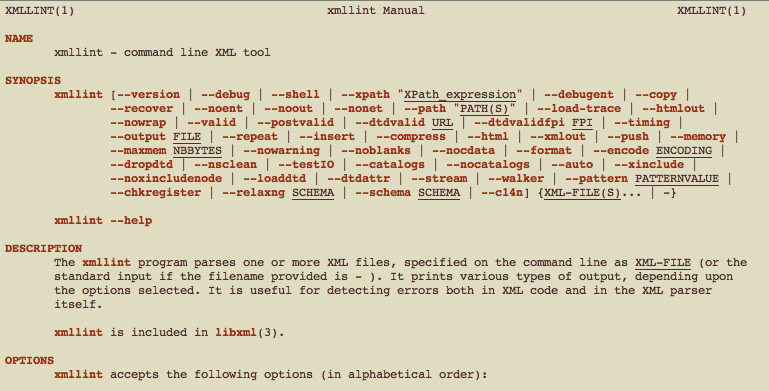
\includegraphics[width=0.95\textwidth]{imgs/xml-XMLlint-man.png}
		\end{center}
	\end{block}

\end{frame}


\begin{frame}
    \frametitle{Fondamenti XML}
    \framesubtitle{eXtensible Markup Language}
    \addtocounter{nframe}{1}

	\begin{block}{XML body}
		Un documento XML è composto da elementi e attributi. 
	   \\ Gli elementi sono la base, le unità fondamentali di qualsiasi documento XML.
    \end{block}

    \begin{block}{Elementi: Sintassi}
    \begin{center}\texttt{<element>content</element>}\end{center}
    \begin{center}\texttt{opening tag: <element>;\\ closing tag: </element>}\end{center}
	\end{block}
	\begin{tiny}
		\textit{Un elemento può contenere testo e/o ulteriori elementi}
	\end{tiny}
	
\end{frame}

\begin{frame}
    \frametitle{Fondamenti XML}
    \framesubtitle{eXtensible Markup Language}
    \addtocounter{nframe}{1}

	\begin{block}{XML Element}
		\textit{Gli elementi XML possono avere diversi tipi di contenuto}:
		\begin{itemize}
			\item contenuto strutturale: solo altri elementi, non testo
			\item contenuto misto: testo e anche altri elementi
			\item contenuto testuale: solo testo, non altri elementi
		\end{itemize}
	\end{block}
	
\end{frame}

\begin{frame}
    \frametitle{Fondamenti XML}
    \framesubtitle{eXtensible Markup Language}
    \addtocounter{nframe}{1}

	\begin{block}{XML Element: note importanti sul nome}
		\begin{itemize}
			\item Gli elementi sono case sensitive.
			\item Gli elementi possono iniziare con una lettera o con un ``\_''.
			\item Un elemento non può iniziare con la stringa \textit{xml}. 
			\item Il tag di apertura e di chiusura devono avere lo stesso nome.
			\item Un tag può essere usato più di una volta.
			\item Un insieme di elementi costituiscono un vocabolario
		\end{itemize}
	\end{block}
\end{frame}




% There are a few important points to remember about XML elements:
% • Element names are case sensitive, which means that, for example, itemnumber,
% itemNumber, and ItemNumber are unique elements.
% • Element names must begin with a letter or the underscore character ( \_ ) and may not
% contain blank spaces. Thus, you cannot name an element Item Number , but you can
% name it Item\_Number .
% • Element names cannot begin with the string xml because that group of ­characters is
% reserved for special XML commands.
% • The name in an element’s closing tag must exactly match the name in the ­opening tag.
% • Element names can be used more than once, so the element names can mean
% different things at different points in the hierarchy of an XML document.

% Element names might be established already if an author is using a particular XML
% vocabulary, such as TEI-XML

% Creating XML Elements
% XML 24
% • To create an XML element, use the syntax
% <element>content</element>
% where element is the name given to the element, content represents the text
% content of the element, <element> is the opening tag, and <
% ­ /element> is the
% closing tag.
% • To create an empty XML element with a single tag, use the following syntax:
% <element />
% • To create an empty XML element with a pair of tags, use the syntax
% <element></element>

\begin{frame}
    \frametitle{Fondamenti XML}
    \framesubtitle{eXtensible Markup Language}
    \addtocounter{nframe}{1}

	\begin{block}{XML Element: empty e nested}
		\begin{itemize}
			\item Un elemento vuoto (\textit{empty}) è un elemento senza contenuto.
			\item Un elemento può contenere altri elementi opportunamente annidati (\textit{nested element}).
		\end{itemize}
	\end{block}

	\begin{block}{XML esempi: empty e nested element}
		\begin{itemize}
			\item \texttt{<element />} \texttt{<element></element>}
			\item \texttt{<choice><sic>testo con errore</sic><cor> testo corretto</cor></choice>}
		\end{itemize}
		
	\end{block}
	
\end{frame}


% ESEMPIO
% <product>
% <productName>Dog Shirt Gift Basket</productName>
% <manufacturer>SJB Pet Boutique</manufacturer>
% <description>Something for every day of the week</description>
% <price>35.99</price>
% <price>26.79</price>
% <productItems>1200, 1201, 1202, 1203, 1204, 1205, 1206
% </productItems>
% </product>

\begin{frame}
    \frametitle{Fondamenti XML}
    \framesubtitle{eXtensible Markup Language}
    \addtocounter{nframe}{1}

	\begin{block}{XML Element: hierarchical relationship}
		\begin{itemize}
			\item Un elemento annidato (\textit{nested}) è un elemento \textit{figlio}, cioè contenuto (annidato) in un ulteriore elemento detto padre/genitore (\textit{parent}).
			\item Gli elementi che sono presenti su uno stesso livello gerarchico (\textit{side by side}) sono detti \textit{sibling element}.
		\end{itemize}
	\end{block}

\end{frame}

\begin{frame}
	\frametitle{Fondamenti XML}
	\framesubtitle{eXtensible Markup Language}
	\addtocounter{nframe}{1}

	\begin{center}
		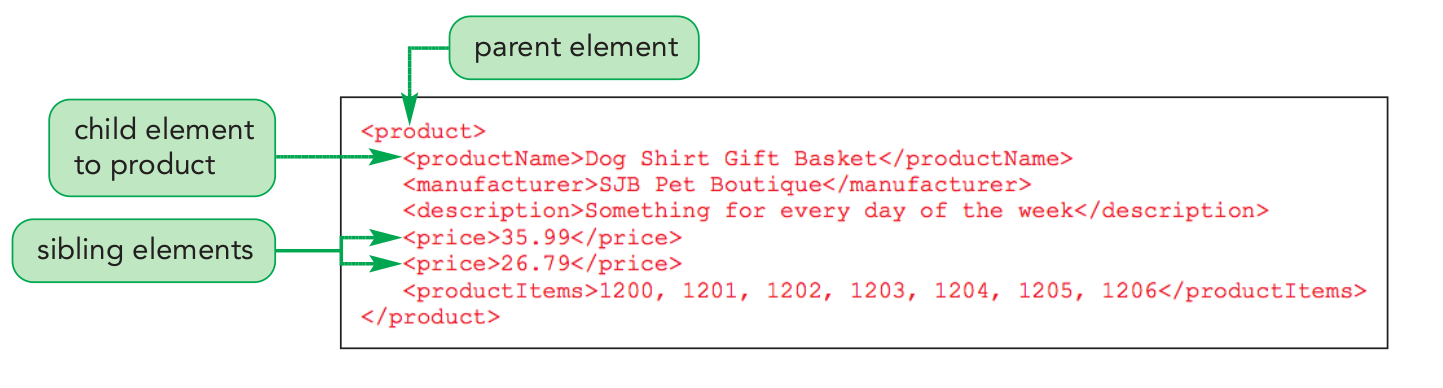
\includegraphics[width=0.95\textwidth]{imgs/XML-Parent-Child-Sibling.png}
    \end{center}
\begin{tiny}\textit{immagine dal libro New Perspectives on XML, 3rd Edition}\end{tiny}

\end{frame}

\begin{frame}
    \frametitle{Fondamenti XML}
    \framesubtitle{eXtensible Markup Language}
    \addtocounter{nframe}{1}

	\begin{block}{XML Element: hierarchical relationship}
		\begin{itemize}
			\item Tutti gli elementi nel body del documento sono figli di uno stesso elemento, chiamato radice (\textit{root}).
			\item Un documento XML deve contenere un elemento root per essere considerato ben formato.
			\item Una gerarchia XML può essere rappresentata tramite un diagramma ad albero.
		\end{itemize}
	\end{block}

\end{frame}

\begin{frame}
    \frametitle{Fondamenti XML}
    \framesubtitle{eXtensible Markup Language}
    \addtocounter{nframe}{1}

	\begin{block}{XML Element: hierarchical relationship cont.}
		\begin{itemize}
			\item Il prologo e i commenti non fanno parte dell'albero del body.
			\item Elementi non annidati correttamente implicano un errore di sintassi nei parser.
			\item Le specifiche XML non consentono di sovrapporre i tag di apertura e di chiusura degli elementi annidati (\textit{no overlap}).
		\end{itemize}
	\end{block}

\end{frame}


\begin{frame}
    \frametitle{Fondamenti XML}
    \framesubtitle{eXtensible Markup Language}
    \addtocounter{nframe}{1}

	\begin{block}{XML Element: hierarchical relationship - Esercizio}
		\begin{center}
			Scrivere e fare il check di un xml non opportunamente annidato
		\end{center}
	\end{block}

\end{frame}

% However, by indenting the code and placing siblings on their own lines, you can visually
% reveal the hierarchy relationships and add a dimension of visual communication to your
% code.

\begin{frame}
    \frametitle{Fondamenti XML}
    \framesubtitle{eXtensible Markup Language}
    \addtocounter{nframe}{1}

	\begin{block}{XML Element: hierarchical relationship as tree structure}
		Un modo rapido e comodo per visualizzare la struttura completa di un documento XML è quello di disegnare attraverso un diagramma ad albero ordinato gli elementi del documento XML.
	\end{block}

\end{frame}

% It would be useful to have a general tree diagram that indicates whether a particular
% child element can occur zero times, once, or several times within a parent

% The symbols ?, *, and + are part of the code used in creating DTDs to validate XML
% documents.

\begin{frame}
	\frametitle{Fondamenti XML}
	\framesubtitle{eXtensible Markup Language}
	\addtocounter{nframe}{1}

	\begin{center}
		%aggiornare immagine

		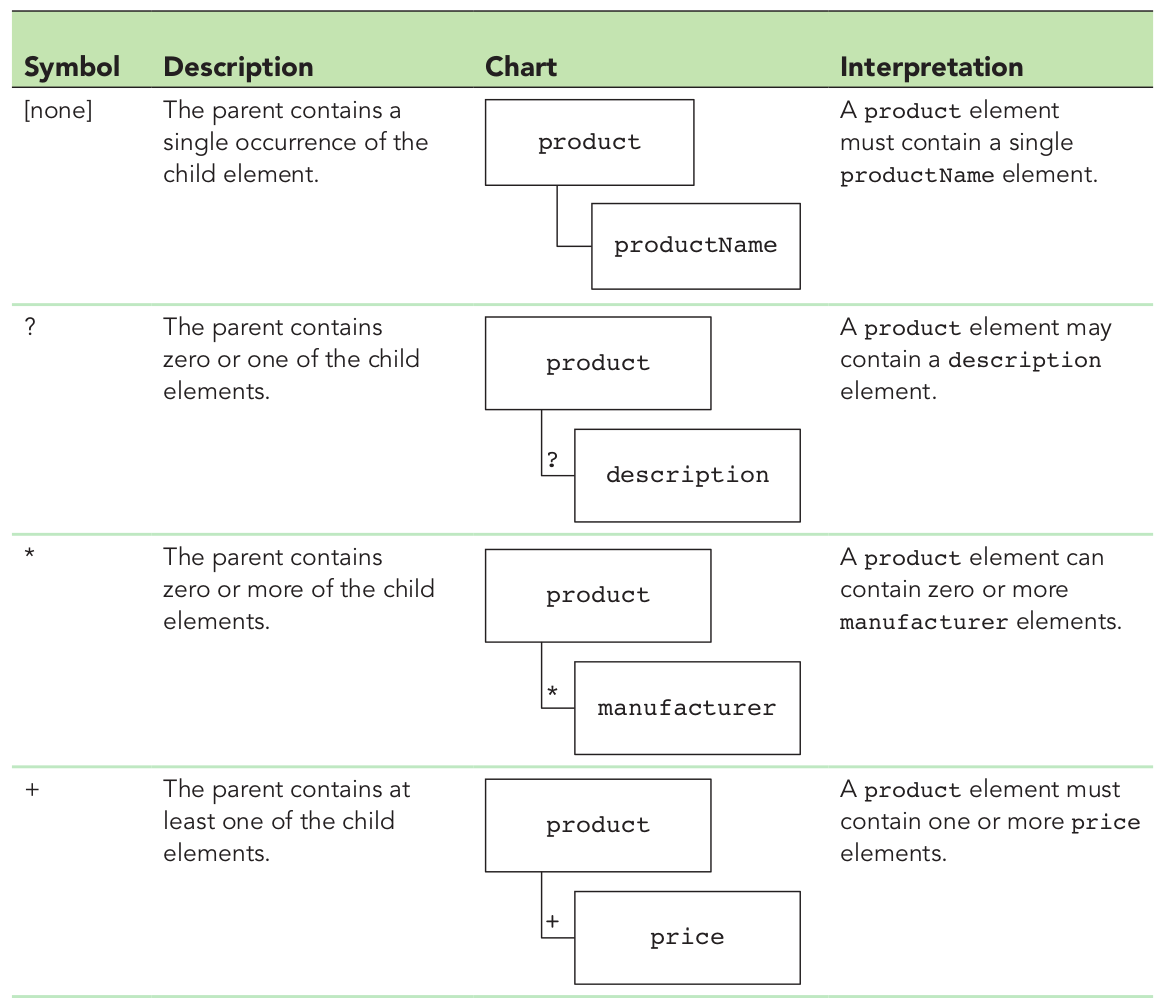
\includegraphics[width=0.8\textwidth]{imgs/xml-parent-child-quantifier.png}
    \end{center}
    
\begin{tiny}\textit{immagine dal libro New Perspectives on XML, 3rd Edition}\end{tiny}

\end{frame}

\begin{frame}
	\frametitle{Fondamenti XML}
	\framesubtitle{eXtensible Markup Language}
	\addtocounter{nframe}{1}

	\begin{center}
		
		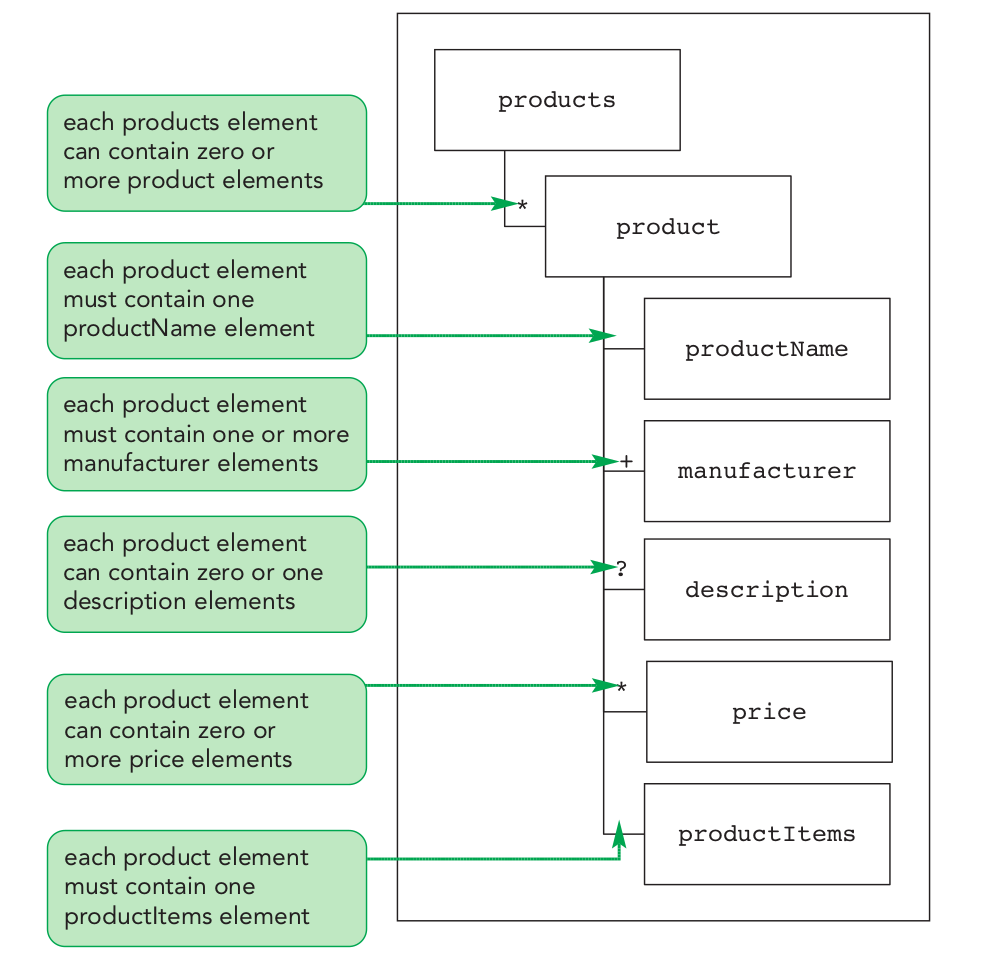
\includegraphics[width=0.7\textwidth]{imgs/xml-parent-child-quantifier2.png}
	\end{center}
\begin{tiny}\textit{immagine dal libro New Perspectives on XML, 3rd Edition}\end{tiny}
\end{frame}


\begin{frame}
    \frametitle{Fondamenti XML}
    \framesubtitle{eXtensible Markup Language}
    \addtocounter{nframe}{1}

	\begin{block}{XML Element: Mixed Content}
		Un elemento può contenere contemporaneamente sia testo sia altri elementi. 
		\\Questo modello di contenuto si chiama Mixed Content ed è ideale per descrivere informazioni text-based (\textbf{dati semi-strutturati)}.
	\end{block}

	\begin{block}{XML Element: Mixed Content}
		\texttt{
			<p><salutation>Salve</salutation> il mio nome è <persName>Angelo</persName></p>
			} 
	\end{block}


\end{frame}

\begin{frame}
    \frametitle{Fondamenti XML}
    \framesubtitle{eXtensible Markup Language}
    \addtocounter{nframe}{1}

	\begin{block}{XML Element: Esercizio}
		Aprire il file XML non ben formato presente nel repository github:
		\begin{itemize}
			\item validarlo con XMLlint
			\item correggerlo (commentando gli errori e le modifiche)
			\item aggiungere un figlio (child) ad un elemento
			\item aggiungere un fratello (sibling) ad un elemento
		\end{itemize}
	\end{block}

\end{frame}


\begin{frame}
    \frametitle{Fondamenti XML}
    \framesubtitle{eXtensible Markup Language}
    \addtocounter{nframe}{1}

	\begin{block}{XML Attributi}
		Gli elementi in un documento XML possono avere uno o più attributi.
		\\ Un attributo descrive una caratteristica dell'elemento in cui appare.
	\end{block}

	\begin{block}{XML Attributi}
		Un attributo ha senso solo all'interno del proprio elemento e non è possibile separarlo da esso in alcun modo.
	\end{block}

\end{frame}


\begin{frame}
    \frametitle{Fondamenti XML}
    \framesubtitle{eXtensible Markup Language}
    \addtocounter{nframe}{1}

	\begin{block}{XML Attributi: valore}
		Un attributo ha due componenti: nome - valore.
		Il valore di un attributo è una stringa e deve essere sempre racchiusa tra apici (singoli o doppi).
	\end{block}

	\begin{block}{XML Attributi: valore}
		\begin{center}
			\texttt{<element attribute=``value''> ... </element>}
			\\\texttt{<element attribute=``value'' />}
			\\\texttt{<element attribute=``value'', attribute2=``value2'' />}
		\end{center}
	\end{block}

\end{frame}

\begin{frame}
    \frametitle{Fondamenti XML}
    \framesubtitle{eXtensible Markup Language}
    \addtocounter{nframe}{1}

	\begin{block}{XML Attributi: restrizioni ai nomi}
		\begin{itemize}
			\item Il nome di un attributo può iniziare con una lettera oppure underscore.
			\item Gli spazi non sono consentiti in un nome di un attibuto.
			\item Il nome di un attributo non pò iniziare con la stringa \textit{xml}.
		\end{itemize}
	\end{block}

	\begin{block}{XML Attributi}
		\begin{itemize}
			\item Il nome degli attributi è \textit{case sensitive}.
			\item L'ordine degli attributi non è significativo.
		\end{itemize}
	\end{block}

\end{frame}


% Esercizio con gli attributi:
% (preso dalla TEI)


% Adding an Attribute to an Element
% • To add an attribute to an element, use the syntax
% <element attribute=”value”> ... </element>
% where element is the name given to the element, attribute is the ­attribute’s
% name, and value is the attribute’s value.
% • To add an attribute to a single-sided tag, use the syntax
% <element attribute=”value” />
% • To specify multiple attributes for a single element, use the syntax
% <element attribute1=”value1” attribute2=”value2” ...> ... </element>
% where attribute1 is the first attribute’s name, value1 is the first attribute’s value,
% attribute2 is the second attribute’s name, value2 is the second ­attribute’s
% value, and so on. Each attribute is separated by a space.



% It’s not always clear when to use an attribute value rather than inserting a new element.
% A general rule of thumb is that if all of the XML tags and their attributes were
% removed from a document, the remaining text should comprise the document’s content
% or information.
% Another rule of thumb is that attributes should be used to describe data, but should
% not contain data themselves.
% Different developers have different preferences, and
% there’s no right answer.

\begin{frame}
    \frametitle{Fondamenti XML}
    \framesubtitle{eXtensible Markup Language}
    \addtocounter{nframe}{1}

	\begin{block}{XML Character and Entity References}
		\begin{itemize}
			\item numeric character reference: \&\#nnn;
			\item character entity reference: \&entity;
		\end{itemize}
	\end{block}

	\begin{block}{XML References}
		\begin{itemize}
			\item \texttt{\&\#65;} (\textit{carattere A})
			\item \texttt{\&amp;} (\textit{carattere \&})
		\end{itemize}
	\end{block}

\end{frame}

% Inserting Character and Entity References
% • To insert a character reference into an XML document, use
% \&\#nnn;
% where nnn is a character reference number from the ISO/IEC character set.
% • To insert an entity reference, use
% \&entity;
% where entity is a recognized entity name.

% Immagine
\begin{frame}
	\frametitle{Fondamenti XML}
	\framesubtitle{eXtensible Markup Language}
	\addtocounter{nframe}{1}

	\begin{center}
			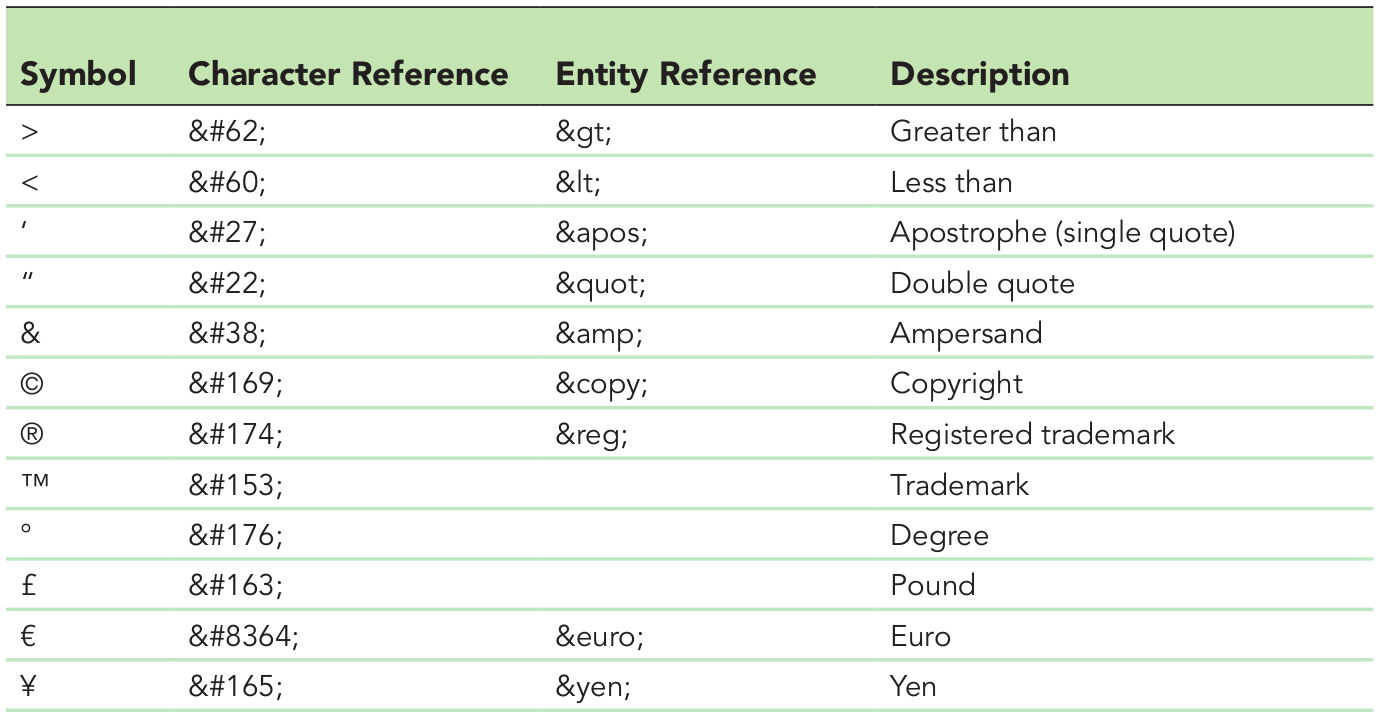
\includegraphics[width=0.95\textwidth]{imgs/xml-Character-Entity.png}
	\end{center}
\begin{tiny}\textit{immagine dal libro New Perspectives on XML, 3rd Edition}\end{tiny}
\end{frame}


\begin{frame}
    \frametitle{Fondamenti XML}
    \framesubtitle{eXtensible Markup Language}
    \addtocounter{nframe}{1}

	\begin{block}{Text Character Parsing}
		Il contenuto testuale di un elemento XML può essere diviso in tre categorie:
		parsed character data, character data, and white space.
	\end{block}

	\begin{block}{Text Character Parsing}
		\begin{itemize}
			\item \texttt{PCDATA}
			\item \texttt{CDATA}
			\item \texttt{White Space}
		\end{itemize}
	\end{block}

\end{frame}


\begin{frame}
    \frametitle{Fondamenti XML}
    \framesubtitle{eXtensible Markup Language}
    \addtocounter{nframe}{1}

	\begin{block}{Parsed Character Data}
		Parsed character data (PCDATA) si riferisce a tutti quei caratteri che XML tratta come parte del codice e quindi vengono interpretati dai parser.
	\end{block}

	\begin{block}{PCDATA}
		\begin{itemize}
			\item XML declaration
			\item Opening tag e  closing tag
			\item Character or entity references
			\item Commenti
		\end{itemize}
	\end{block}

\end{frame}

% The presence of PCDATA can cause unexpected errors to occur within a document
% This means that symbols such as \&, <, or >, which are all used in ­creating
% markup tags or entity references, are extracted and the appropriate content is used in your program.

\begin{frame}
    \frametitle{Fondamenti XML}
    \framesubtitle{eXtensible Markup Language}
    \addtocounter{nframe}{1}

	\begin{block}{Parsed Character Data}
		La presenza di contenuti di tipo PCDATA può causare errori inaspettati.
	\end{block}

	\begin{block}{XML PCDATA}
		Caratteri speciali che sono utilizzati dalla specifica XML come \texttt{\&, <, >} non possono essere utilizzati come contenuto testuale.
	\end{block}

\end{frame}


% Character Data

\begin{frame}
    \frametitle{Fondamenti XML}
    \framesubtitle{eXtensible Markup Language}
    \addtocounter{nframe}{1}

	\begin{block}{Character Data}
		I dati di tipo ``Character Data'' non vengono interpretati dal parser XML.
		\\ La sequenza di caratteri viene trattata come puro contenuto.
		\\In definitiva una sezione \textit{CDATA} è un blocco di testo.
	\end{block}

	\begin{block}{XML CDATA: sintassi}
		\begin{center}
			\texttt{
				 <![CDATA [
					 \\character data
					 \\]]>
			}
		\end{center}
	\end{block}

\end{frame}


%A CDATA section

\begin{frame}
    \frametitle{Fondamenti XML}
    \framesubtitle{eXtensible Markup Language}
    \addtocounter{nframe}{1}

	\begin{block}{Character Data}
		Le sezioni di testo CDATA possono essere inserite in qualsiasi parte del documento XML.
		\\ Utile per inserire una sezione di testo com molti caratteri speciali.
	\end{block}

\end{frame}

\begin{frame}
    \frametitle{Fondamenti XML}
    \framesubtitle{eXtensible Markup Language}
    \addtocounter{nframe}{1}

	\begin{block}{CDATA: qualche vincolo}
		\begin{itemize}
			\item Non è possibile inserire commenti in una sezione CDATA.
			\item Non è possibile annidare sezioni CDATA. 
			\item Non possono essere vuote.
			\item i simboli ``]]'' non sono ammessi.
		\end{itemize}
	\end{block}

\end{frame}


\begin{frame}
    \frametitle{Fondamenti XML}
    \framesubtitle{eXtensible Markup Language}
    \addtocounter{nframe}{1}

	\begin{block}{Esempio ed esercizio}
		Inserire all'interno di un tag un frammento di codice HTML
	\end{block}

	\begin{block}{CDATA: esempio}
		\begin{center}
			\texttt{
			<htmlCode>
			 <![CDATA[
			 		<h1>Capitolo Primo</h1>
			 		<h2>Sezione Seconda</h2>
			 	]]>
			 </htmlCode>
			 }
		\end{center}
	\end{block}

\end{frame}


% White Space

\begin{frame}
    \frametitle{Fondamenti XML}
    \framesubtitle{eXtensible Markup Language}
    \addtocounter{nframe}{1}

	\begin{block}{White Space: esempio}
		\begin{itemize}
			\item Gli spazi bianchi sono ignorati quando sono tra i tag.
			%White space is ignored when it is the only character data between element tags
			\item Gli spazi bianchi sono ignorati all'interno del prologo e dell'epilogo e all'interno dei tag. 
			%White% space is ignored within a document prolog and epilog, and within any element tags
			\item Gli spazi bianchi inseriti nel valore di un attributo sono trattati come parte del contenuto.
			%White space within an attribute value is treated as part of the attribute value
			\item Non vengono strippati gli spazi all'interno del contentuto testuale degli elementi.
			%no white space ­stripping occurs for element content, which means that the content of the XML element
		\end{itemize}
	\end{block}

	\begin{tiny}
		I white space sono caratteri non stampabili
	\end{tiny}


\end{frame}

% Inserting a Processing Instruction

\begin{frame}
    \frametitle{Fondamenti XML}
    \framesubtitle{eXtensible Markup Language}
    \addtocounter{nframe}{1}

	\begin{block}{Processing Instruction}
		Una \textit{processing instruction} è un comando, una direttiva, che indica al parser XML in che modo elaborare e trattare tutto o parte del documento XML.
	\end{block}

	\begin{block}{Processing Instruction: sintassi}
		\begin{center}
			\texttt{<?target instruction ?>}
			\\\texttt{<?xml-stylesheet type=”text/css” href=”main.css” media=”all” ?>}
		\end{center}
	\end{block}
\begin{tiny}
    \textit{Molteplici processing instruction possono co-esistere all'interno di un unico documento XML.}
\end{tiny}
    
	% Multiple processing instructions can exist within the same XML document for different
% media types

\end{frame}



\begin{frame}
    \frametitle{Fondamenti XML}
    \framesubtitle{eXtensible Markup Language}
    \addtocounter{nframe}{1}

	\begin{block}{Processing Instruction: sintassi}
		\begin{center}
			\texttt{<?target instruction ?>}
			\\\texttt{<?xml-stylesheet type=”text/css” href=”main.css” media=”all” ?>}
		\end{center}
	\end{block}


	\begin{block}{Processing Instruction}
		 \textbf{Target}: identifica il tool al quale la processing instruction è diretta.
		 \\\textbf{Instruction}: identifica le informazioni che il documento passa al parser per essere elaborate. Le istuzioni hanno la forma degli attributi (nome-valore).
	\end{block}

\end{frame}

% Working with Namespaces

% involves two steps:
% 1. Declare the namespace.
% 2. Identify the elements and attributes within the document that belong to that
% namespace.


\begin{frame}
    \frametitle{Fondamenti XML}
    \framesubtitle{eXtensible Markup Language}
    \addtocounter{nframe}{1}

	\begin{block}{Namespaces}
		Un namespace può essere visto come una collezione di elementi e attributi e un insieme di regole che ne determinano la struttura e il contenuto.
	\end{block}

	\begin{block}{Namespaces}
		\begin{center}
			\texttt{<element xmlns:prefix=”uri”> ... </element>}
			\\\texttt{<element xmlns=”uri”> ... </element>}
			\\\texttt{<tei:TEI xmlns:tei=``http://www.tei-c.org/ns/1.0''>}
			\\\texttt{<TEI xmlns=``http://www.tei-c.org/ns/1.0''>}
		\end{center}
	\end{block}

\end{frame}

% (URI)—a text string that uniquely identifies a resource.
% The purpose of a URI is simply to provide a
% unique string of characters that identify a resource.
% One version of a URI is the Uniform Resource Locator (URL)
% URLs serve as a built-in mechanism on the web for generating unique addresses
% Note that although a URI
% doesn’t actually need to point to a real site on the web, it’s often helpful to place
% documentation at the site identified by a URI so users can go there to learn more
% about the XML vocabulary being referenced.


% The number of namespace attributes that can be declared within an element is
% unlimited.

% root element so that each namespace is available to all
% elements within the document

% You can declare a default namespace by omitting the prefix in the namespace ­declaration.
% Any descendant element or attribute is then considered part of this namespace unless a
% different namespace is declared within one of the child elements.


\begin{frame}
    \frametitle{Fondamenti XML}
    \framesubtitle{eXtensible Markup Language}
    \addtocounter{nframe}{1}

	\begin{block}{Namespaces}
		Un namespace viene ereditato da tutti gli elementi discendenti dell'elemento in cui esso è stato dichiarato.
	\end{block}

	\begin{block}{Namespaces}
		Generalmente si dichiarano tutti i namespace nell'elemento root così da avere a disposizione tutti gli elementi dei vari namespace in tutto il documento XML
	\end{block}

\end{frame}

% esempio di dichiarazione di vari namespace in un documento XML

% Declaring a Namespace
% • To declare a namespace for an element within an XML document, add the
% xmlns:prefix attribute to the opening tag of the element using the syntax
% <element xmlns:prefix=”uri”> ... </element>
% where element is the element in which the namespace is declared, prefix is the
% namespace prefix, and uri is the URI of the namespace.
% • To declare a default namespace, add the xmlns attribute without specifying a prefix,
% as follows:
% <element xmlns=”uri”> ... </element>

% immagini di riepilogo












% Attributes can only store a value, while elements can also store child elements and attributes.
% An element can appear more than once within a parent node, but an attribute can appear only once. The order of attributes is not significant and there is no way to control the order of attributes in XSD. If the attribute is present the default value is not assigned, even if the value of the attribute is an empty string.
% the default value of elements is assigned only when the element is present and is empty
% Elements are mandatory by default while attributes are optional by default.


%Both HTML and XML use tags in similar ways, often creating distinctly hierarchical structures to present data to users.

% Like HTML documents, XML documents can be created and viewed with a basic text editor such as Notepad or TextEdit. More sophisticated XML editors are available, and using them can make it easier to design and test documents.




% tanti vocabolari XML
% Bioinformatic Sequence Markup
% Language (BSML) Coding of bioinformatic data
% Extensible Hypertext Markup Language
% (XHTML) HTML written as an XML application
% Mathematical Markup Language
% (MathML) Presentation and evaluation of mathematical equations
% and operations
% Music Markup Language (MML) Display and organization of music notation and lyrics
% Weather Observation Definition
% Format (OMF) Distribution of weather observation reports, forecasts, and
% advisories
% Really Simple Syndication (RSS) Distribution of news headlines and syndicated columns
% Synchronized Multimedia Integration
% Language (SMIL) Editing of interactive audiovisual presentations ­involving
% streaming audio, video, text, and any other media type
% Voice Extensible Markup Language
% (VoiceXML) Creation of audio dialogues that feature synthesized
% speech, digitized audio, and speech recognition
% Wireless Markup Language (WML) Coding of information for smaller-screened devices, such
% as PDAs and cell phones

\begin{frame}
    \frametitle{Elementi XML}
    \framesubtitle{Conclusioni}
    \addtocounter{nframe}{1}

    \begin{block}{XML per rappresentare il testo}
    %\begin{center}\texttt{<!DOCTYPE root PUBLIC “id” “uri”>}\end{center}
    %\begin{center}\texttt{standard//owner//description//language}\end{center}
    %\begin{center}\texttt{-//W3C//DTD XHTML 1.0 Strict//EN}\end{center}
        \begin{itemize}
            \item I markup language per supportare la rappresentazione, memorizzazione, pubblicazione di un testo.
            \item XML è un markup language flessibile e potente.
        \end{itemize}

        \begin{itemize}
            \item le istruznioni dei markup language sono per lo più dichiarazioni indicando particolari funzioni del dato.
            \item le istruznioni sono etichette visibili.
        \end{itemize}
        
    \end{block}

\end{frame}

\begin{frame}
    \frametitle{Elementi XML}
    \framesubtitle{Conclusioni}
    \addtocounter{nframe}{1}

    \begin{block}{XML per rappresentare il testo}
    %\begin{center}\texttt{<!DOCTYPE root PUBLIC “id” “uri”>}\end{center}
    %\begin{center}\texttt{standard//owner//description//language}\end{center}
    %\begin{center}\texttt{-//W3C//DTD XHTML 1.0 Strict//EN}\end{center}
        \begin{itemize}
            \item Una sintassi e una grammatica regolano l'applicabilità del linguaggio di marcatura
            \item Sintassi: documento well formed (ben formato)
            \item Grammatica: documento valido
        \end{itemize}

    \end{block}

\end{frame}


\begin{frame}
    \frametitle{Elementi XML}
    \framesubtitle{Conclusioni}
    \addtocounter{nframe}{1}

    \begin{block}{XML per rappresentare il testo}
    %\begin{center}\texttt{<!DOCTYPE root PUBLIC “id” “uri”>}\end{center}
    %\begin{center}\texttt{standard//owner//description//language}\end{center}
    %\begin{center}\texttt{-//W3C//DTD XHTML 1.0 Strict//EN}\end{center}
        \begin{itemize}
            \item XML deriva dal linguaggio SGML.
            \item XML è una specifica del consorzio W3C.
            \item XML è un meta-linguaggio.
            \item XML è plain text.
            \item XML è portabile.
        \end{itemize}

    \end{block}

\end{frame}

\begin{frame}
    \frametitle{Elementi XML}
    \framesubtitle{Conclusioni}
    \addtocounter{nframe}{1}

    \begin{block}{XML per rappresentare il testo}
    %\begin{center}\texttt{<!DOCTYPE root PUBLIC “id” “uri”>}\end{center}
    %\begin{center}\texttt{standard//owner//description//language}\end{center}
    %\begin{center}\texttt{-//W3C//DTD XHTML 1.0 Strict//EN}\end{center}
        \begin{itemize}
            \item XML definisce markup dichiarativi e descrittivi.
            \item XML ha un modello dati ad albero ordinato.
            \item XML può avere associato un tipo di documento (DTD) o uno schema (XSD).
        \end{itemize}

    \end{block}

\end{frame}
